\documentclass[journal]{IEEEtran}
\usepackage{amsmath,amssymb}
\usepackage{graphicx}
\usepackage{booktabs}
\usepackage{multirow}
\usepackage[numbers,sort&compress]{natbib}
\usepackage{xcolor}
\usepackage[colorlinks=true,linkcolor=blue!50!black,citecolor=blue!50!black,urlcolor=blue!50!black]{hyperref}
\graphicspath{{../figures/}}

\begin{document}
\title{Learned Bias Correction for Surface-Area\\ Estimation from CT-like Voxel Data}
\author{Manas Jain}
\maketitle

\begin{abstract}
Measuring the surface area of an object from a CT scan is harder than it looks, because the scan is a
grid of small cubes (voxels) and the true surface passes between them. Counting the exposed faces of
the voxels gives an area about 50\% too large at every resolution. Marching cubes, which fits a
triangle mesh to the data, is closer, but its error depends on how curved the object is and how noisy
the scan is. We built 2,400 synthetic shapes from seven families whose true surface area is known to
better than 0.01\%, and turned them into 14,400 CT-like volumes at $32^3$ and $64^3$ voxels with three
noise levels. We then trained models to predict, for each object, how much the marching-cubes area
should be corrected: a Random Forest on ten simple shape measurements, a 3D convolutional neural
network (CNN) and a PointNet. On test shapes that none of the models had seen, marching cubes has an
average error of 4.78\% ($32^3$) and 3.52\% ($64^3$). The best corrections bring this down to 0.68\%
(3D CNN, $32^3$) and 0.18\% (Random Forest, $64^3$), and stay below 2\% on two shape families left out of
training altogether. The simple Random Forest does as well as the CNN overall, the CNN is better only
for objects smaller than 16 voxels, and no method can recover structures thinner than about two voxels.

\end{abstract}

\begin{IEEEkeywords}
Computed tomography, surface area, marching cubes, partial-volume effect, deep learning, 3D CNN,
PointNet, synthetic data.
\end{IEEEkeywords}

\section{Introduction}\label{sec:intro}
Surface area is one of the most requested measurements in X-ray computed tomography (CT) of materials
and parts. It controls reaction rates in catalysts, flow in porous media and the quality of additively
manufactured lattices. It is usually measured from the reconstructed voxel volume, either by counting
the exposed faces of segmented voxels or by extracting a triangle mesh with marching cubes
\citep{lorensen1987} and summing the triangle areas.

Both routes are biased. Counting voxel faces measures the area of a staircase, which is about 50\%
larger than the true surface at every resolution. Marching cubes on a thresholded (binary) volume is
better, but its error does not vanish as the voxels get smaller \citep{kenmochi2000,svane2013}.
Marching cubes on the greyscale volume is accurate for clean, well-resolved data, but real CT volumes
are noisy and many structures are only a few voxels across. Because the error depends on resolution,
noise, curvature and thin features at the same time, a single correction factor cannot remove it.

This work builds a synthetic CT-like dataset with exactly known surface areas and trains models that
predict a correction to the greyscale marching-cubes area for each object, so that learning acts as a
correction layer on top of the classical measurement rather than replacing it.


\section{Problem, Objectives and Motivation}\label{sec:problem}
\paragraph{Problem.} Given a CT-like greyscale volume of a single object on an $N^3$ grid, estimate the
area of the object's true, continuous surface. The volume is degraded by the finite voxel size
(partial-volume averaging), by the scanner blur and by noise.

\paragraph{Objectives.} (1) Build shapes with reference areas accurate to better than $10^{-4}$, so that
the reference adds no error of its own. (2) Measure the error of voxel-face counting and three
marching-cubes variants across resolution and noise. (3) Train a 3D CNN and a PointNet to correct the
greyscale marching-cubes area, and compare them with a per-regime lookup table and a Random Forest.
(4) Test the corrections on shape families never seen in training. (5) State when a learned correction
is worth using.

\paragraph{Why this matters.} A 5\% error in surface area is large compared with the effects such
measurements are used to detect, for example differences between catalyst batches or the deviation of
a printed lattice from its design. Errors of this size are typical for small or noisy objects
(Section~\ref{sec:results}). A correction learned once on synthetic data is cheap to apply to every new
object.


\section{Theory}\label{sec:theory}
This section explains why each classical method gets the area wrong, and by how much. In short:
counting voxel faces measures a staircase instead of the real surface, so it is always too high;
marching cubes on a black-and-white volume can only build a few triangle directions, so it leaves a
small zig-zag that never goes away; and marching cubes on the greyscale volume is very good on flat
surfaces but slightly too small on curved ones (because the scan blurs the surface) and too large on
noisy ones. Knowing where each error comes from tells us what a correction model has to learn.

\subsection{Voxel-face counting}
Consider a planar piece of surface with unit normal $\mathbf n=(n_x,n_y,n_z)$. Its digital
(staircase) version is made of voxel faces normal to the three axes, and the total area of the faces
normal to axis $i$ equals the projection of the true area onto the plane perpendicular to that axis.
The face-count area per unit true area is therefore
\begin{equation}
  r(\mathbf n) = |n_x| + |n_y| + |n_z|, \qquad 1 \le r \le \sqrt3 .
\end{equation}
It equals 1 only for axis-aligned surfaces (Fig.~\ref{fig:facetheory}). For normals distributed
uniformly on the sphere each component is uniform on $[-1,1]$, so $\mathbb E|n_i| = 1/2$ and
$\mathbb E\,r = 3/2$. The face count of a randomly oriented smooth object thus overestimates its area by
50\%, and since $r$ does not depend on the voxel size, refining the grid does not help. On a clean sphere
at $128^3$ we measure $+50.03\%$.

\begin{figure}[t]
  \centering
  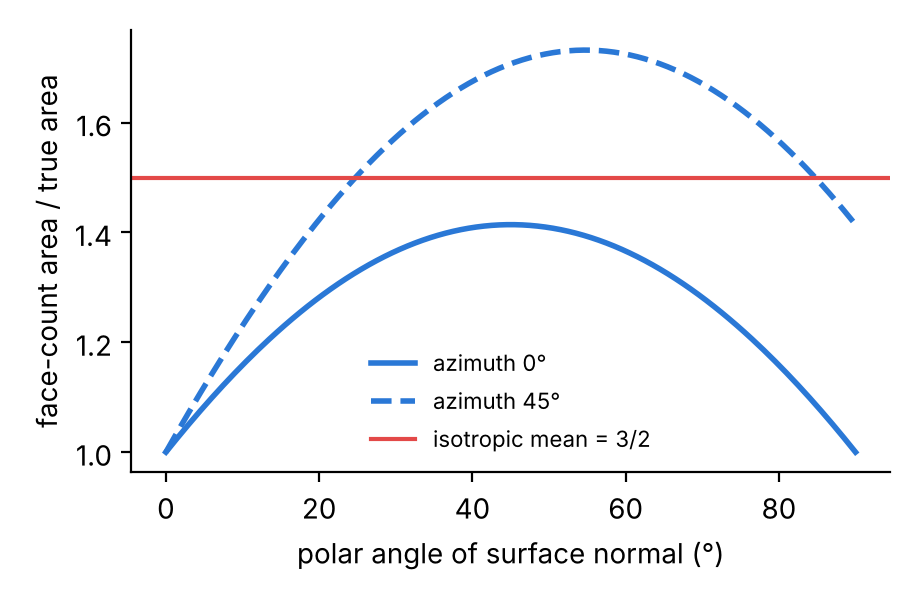
\includegraphics[width=0.52\linewidth]{face_count_theory.png}
  \caption{Face-count area per unit true area, $|n_x|+|n_y|+|n_z|$, for a plane whose normal makes the
  given polar angle with the $z$ axis, at azimuth 0° and 45°. The isotropic average is $3/2$.}
  \label{fig:facetheory}
\end{figure}

\subsection{Marching cubes on binary and greyscale volumes}
Marching cubes \citep{lorensen1987} places triangle vertices on the edges of each $2\times2\times2$
cell where the image crosses the iso-level. On a binary volume the crossing is always at the edge
midpoint, so only a finite set of triangle orientations can occur, and the mesh approximates a plane
of arbitrary orientation by a small-scale zig-zag whose excess area depends on the orientation but not
on the voxel size. Using smaller voxels makes the zig-zag finer but not flatter, so the area error does
not go to zero as the grid is refined \citep{kenmochi2000,svane2013}. On clean spheres we
measure $+7.3\%$ at $16^3$, rising to $+8.8\%$ at $128^3$.

On a greyscale volume the vertex position is interpolated from the partial-volume intensities, so
the mesh can follow the surface between voxel centres. For a flat surface the half-intensity level of
the blurred image lies exactly on the true surface. For a curved surface it does not: blurring spreads
the object's intensity outwards over a larger volume, so the half-intensity surface ends up slightly
inside the true one, and more so where the surface bends sharply. The result is an area that is a
little too small. For a sphere of radius $R$ voxels the expected error is about $-2\sigma^2/R^2$, where
$\sigma^2$ measures the total blur ($\sigma^2 \approx 0.44$ voxel$^2$ in our data). This predicts
$-0.56\%$ for a sphere on a $32^3$ grid, and we measure $-0.62\%$. The error shrinks quickly as objects
get larger, but extra smoothing (often used to remove noise) makes it about three times bigger. The
derivation and the full comparison are in Appendix~\ref{app:curvature}.

\subsection{Effect of noise}
Additive noise with standard deviation $\sigma_n$ has two effects on marching cubes. First, it perturbs
the iso-crossing positions near the surface. A randomly perturbed surface has more area than the
smooth one, since the area element $\sqrt{1+|\nabla\eta|^2}\ge1$ for any height perturbation $\eta$,
so this bias is always positive. Second, background voxels exceed the iso-level by chance with
probability $p = Q(0.5/\sigma_n)$, where $Q$ is the Gaussian tail function, and object voxels fall below
it with the same probability. Each such voxel becomes a tiny closed surface or cavity. For
$\sigma_n = 0.15$, $p = Q(3.33) \approx 4.3\times10^{-4}$, which predicts about 112 spurious components on
a $64^3$ grid and 14 on a $32^3$ grid. These specks can be counted with the Euler number of the
thresholded volume (roughly, the number of separate pieces and cavities minus the number of tunnels),
since each speck adds one to it. The measured Euler numbers at this noise level are indeed about 100 to
125 at $64^3$. For $\sigma_n = 0.05$, $p = Q(10)$ is negligible and only the surface roughening remains.
Gaussian smoothing removes most of this noise, but as explained above it also shrinks curved surfaces,
and it erases structures thinner than about $2\sigma_s$ entirely (we observe this for the thinnest tori
on the $32^3$ grid, where the smoothed volume never reaches the iso-level).

The upshot is that greyscale marching cubes has a negative, curvature-driven bias that grows at low
resolution, plus a positive, noise-driven bias that grows with $\sigma_n$ and with the number of
voxels. The two can partly cancel, which is why a single correction factor cannot fix both.

\subsection{Reference surface area}
Measuring the error of each method needs the true area of every shape. Spheres, cylinders, tori and
ellipsoids have exact formulas. Random blobs and superellipsoids do not, so their area is computed
numerically: the surface is covered with a very fine triangle mesh at two levels of detail (about
82,000 and 328,000 triangles), and the two results are combined to cancel the leading error term. The
remaining error is below 0.01\% for every shape, far smaller than the errors being measured. The
formulas are given in Appendix~\ref{app:reference}.

\subsection{Learning target}
All models predict
\begin{equation}
  y = \log\frac{A_\text{true}}{A_\text{MC}},
\end{equation}
where $A_\text{MC}$ is the greyscale marching-cubes area, and the final estimate is
$\hat A = A_\text{MC}\,e^{\hat y}$. The target is dimensionless, so it does not depend on the size of the
object, and it is invariant to rotations and translations of the object. This lets the training data
be augmented exactly with the 48 symmetries of the cube (axis permutations and reflections), which
permute voxels without interpolation and leave the true area unchanged.


\section{Previous Work}\label{sec:previous}
\paragraph{Mesh-based measurement.} Marching cubes \citep{lorensen1987} is the standard way to extract
an iso-surface from a voxel volume; we use the topologically consistent variant of \citet{lewiner2003}
as implemented in scikit-image \citep{vanderwalt2014}. \citet{nystrom2002} compared areas of digital
(voxel-face) surfaces and triangulated surfaces on phantoms and real objects and found the
triangulated areas considerably more accurate, with errors decreasing as the voxel size decreased.

\paragraph{Local estimators and multigrid convergence.} A large body of work in digital geometry
estimates surface area from binary volumes by assigning a weight to each local $2\times2\times2$
configuration. \citet{mullikin1993} derived optimal weights for digitized planes, and
\citet{windreich2003} and \citet{lindblad2005} optimised local configuration weights to minimise the
bias for isotropically oriented surfaces. A central theoretical question is multigrid convergence,
i.e.\ whether the estimate converges to the true area as the grid is refined. \citet{kenmochi2000}
showed that local polyhedrization schemes such as marching cubes on binary data are not multigrid
convergent even for spheres, cubes and cylinders, and \citet{svane2013} proved that no local digital
algorithm for surface area is multigrid convergent on the class of convex polytopes.
\citet{ziegel2010} studied design-based surface-area estimation from digitizations with random grid
placement. \citet{klette2004} give a general account. These results explain why the binary estimators
in this work keep a resolution-independent bias, and they motivate using greyscale information.

\paragraph{Learning-based estimation.} Deep networks operating directly on voxel grids
\citep{maturana2015} and on unordered point sets \citep{qi2017} are established tools for 3D shape
analysis. For CT of porous materials, \citet{rabbani2020} trained a convolutional network to predict a
range of morphological, hydraulic, electrical and mechanical properties of porous samples from 3D
images in a fraction of the time of image-based simulation. Random Forests \citep{breiman2001} on
hand-crafted descriptors remain a strong baseline for small tabular problems.

\paragraph{Gap.} The work above either derives fixed estimators for binary data or learns global
properties of complex microstructures, where an exact ground truth is not available. We did not find a
study that measures how much a learned model reduces surface-area bias relative to marching cubes
against an exact reference, separately for resolution, noise level and unseen shape families, and that
compares deep models with a calibrated feature-based baseline. That comparison is the subject of this
work.


\section{Method}\label{sec:method}
\subsection{Data}
Table~\ref{tab:families} lists the seven shape families. Five are used for training: spheres (150 shapes), ellipsoids (350), capped cylinders
(300), tori (300) and smooth random blobs (900), the last being star-shaped surfaces built from six
low-frequency waves on the sphere. Two families are held out for testing only: superellipsoids (200),
with pointed tips or box-like rounded edges, and rough blobs (200), which add ten high-frequency waves.
Each shape is scaled to fill 35--100\% of the grid (diameters 9.8 to 60 voxels), randomly rotated and
shifted by a sub-voxel offset. The volume is formed by a simple CT model: partial-volume occupancy
computed with $5\times5\times5$ supersampling, a Gaussian blur with $\sigma=0.6$ voxel, and Gaussian noise
with $\sigma_n\in\{0, 0.05, 0.15\}$ relative to unit contrast, stored as 8-bit integers. Every shape is
rendered at $N=32$ and $64$ and all three noise levels, giving six volumes per shape and 14,400 in total.
The split is by shape (70/15/15 within each training family, fixed seed 51), so all six volumes of a
shape stay together: 1,400 training, 299 validation and 301 test shapes, plus the 400 held-out shapes.
Figure~\ref{fig:slices} shows one shape at both resolutions and all noise levels.

\begin{table*}[t]
  \centering\small
  \caption{Shape families. Parameters are drawn uniformly from the given ranges; all shapes are
  normalised to maximum extent 1 before placement.}
  \label{tab:families}
  \begin{tabular}{llrl}
    \toprule
    Family & Role & Shapes & Parameters \\
    \midrule
    Sphere & train & 150 & radius 1 \\
    Ellipsoid & train & 350 & $a=1$, $b,c\in[0.35,1]$ \\
    Cylinder (capped) & train & 300 & radius $\in[0.3,0.85]$, half-height $\sqrt{1-\rho^2}$ \\
    Torus & train & 300 & $r/R\in[0.2,0.6]$, $R+r=1$ \\
    Smooth blob & train & 900 & 6 waves, $\omega\in[1,3]$, s.d.\ of $\log r\in[0.15,0.30]$ \\
    \midrule
    Superellipsoid & held out & 200 & $b,c\in[0.45,1]$; $p\in[1.5,1.8]$ (40\%) or $[3,6]$ (60\%) \\
    Rough blob & held out & 200 & smooth blob $+$ 10 waves, $\omega\in[8,14]$, s.d.\ $\in[0.02,0.05]$ \\
    \bottomrule
  \end{tabular}
\end{table*}

\begin{figure}[t]
  \centering
  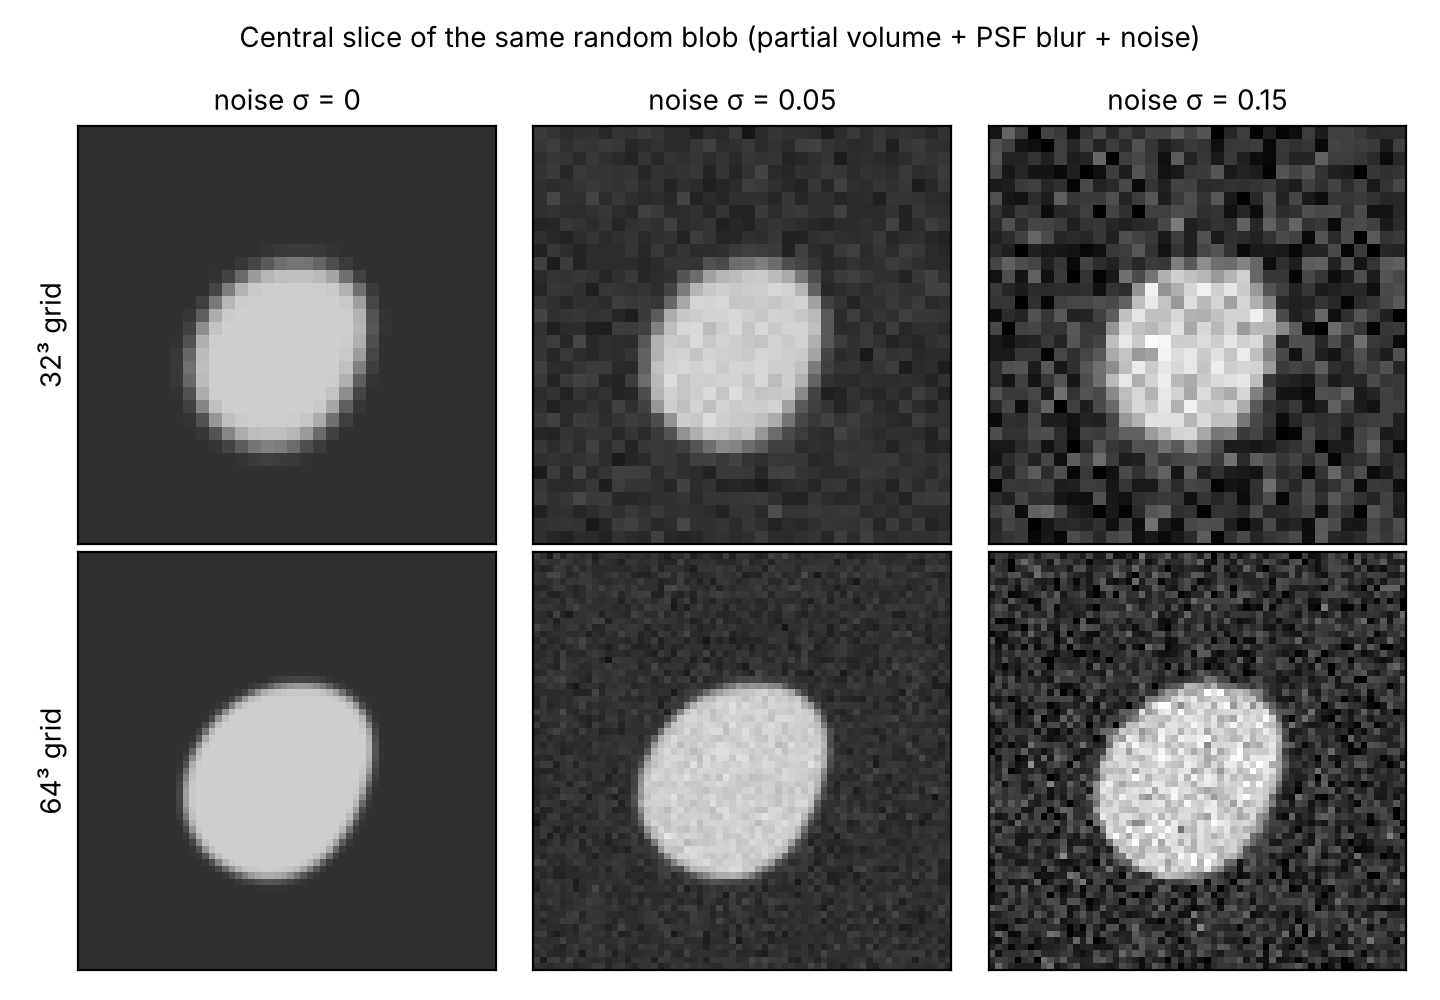
\includegraphics[width=\columnwidth]{example_slices.png}
  \caption{Central slice through the same random blob at both resolutions and all three noise levels.}
  \label{fig:slices}
\end{figure}

\begin{figure}[t]
  \centering
  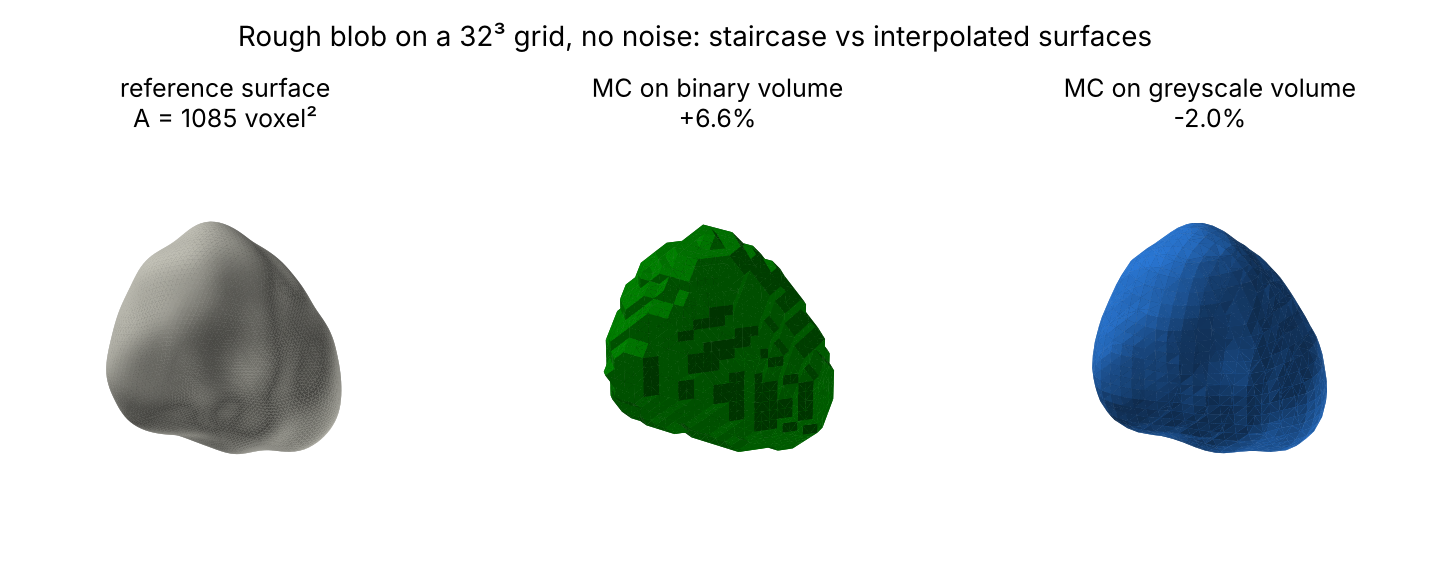
\includegraphics[width=\columnwidth]{example_meshes.png}
  \caption{Reference surface of a rough blob and the marching-cubes meshes from its clean $32^3$ volume.
  The binary mesh is a staircase; the greyscale mesh is smooth but loses the finest detail.}
  \label{fig:meshes}
\end{figure}

\subsection{Estimators}
\textbf{Classical:} voxel-face counting after thresholding at 0.5; marching cubes on the thresholded
(binary) volume; marching cubes on the greyscale volume at iso-level 0.5; and marching cubes after
Gaussian smoothing with $\sigma_s=1$ voxel (Fig.~\ref{fig:meshes}). \textbf{MC + lookup} multiplies the
greyscale area by the median training correction for the same resolution and noise level; it is given
the true noise level, so any learned model has to beat it to show that it does more than apply an
average. \textbf{Random Forest} \citep{breiman2001} (400 trees) predicts $y$ from ten simple
measurements: the greyscale area relative to $N^2$, the ratios of the face, binary and smoothed areas to
it, a compactness term, two aspect ratios, the Euler number of the thresholded volume, a noise estimate
and $N$.

\textbf{3D CNN:} five convolutional blocks with 16 to 256 channels, batch normalisation, ReLU and max
pooling, then global average and max pooling and a 128-unit head (3.59M parameters).
\textbf{PointNet} \citep{qi2017}: 2,048 points sampled on the greyscale mesh, a shared MLP up to 1,024
features, max pooling and a 512--128 head (0.74M parameters), with random rotations instead of the
alignment network. Both are trained per resolution with a Huber loss on $y/0.05$, AdamW, a one-cycle
learning-rate schedule \citep{smith2019} with peak $10^{-3}$, batch size 32, up to 40 epochs (15 for the
CNN at $64^3$) and early stopping on the validation error, using PyTorch \citep{paszke2019} on an
Apple-silicon laptop. We report the mean absolute percentage error (MAPE) and the mean signed error
(bias) of $\hat A/A_\text{true}-1$ on held-out shapes only.


\section{Results}\label{sec:results}
All results are on shapes not used for training or model selection: the test split (301 shapes, 903
volumes per resolution) and the two held-out families (200 shapes each). Table~\ref{tab:main} gives the
overall picture.

\begin{table*}[t]
  \centering\footnotesize
  \caption{Surface-area error (\%) on held-out shapes, all noise levels pooled. MAPE: mean absolute error; bias: mean signed error. The two right-hand blocks are shape families never seen in training (MAPE). Best value per column in bold.}
  \label{tab:main}
  \setlength{\tabcolsep}{3.5pt}
  \begin{tabular}{lrrrrrrrr}
    \toprule
    & \multicolumn{2}{c}{Test MAPE} & \multicolumn{2}{c}{Test bias} & \multicolumn{2}{c}{Superellipsoid} & \multicolumn{2}{c}{Rough blob} \\
    \cmidrule(lr){2-3}\cmidrule(lr){4-5}\cmidrule(lr){6-7}\cmidrule(lr){8-9}
    Method & $32^3$ & $64^3$ & $32^3$ & $64^3$ & $32^3$ & $64^3$ & $32^3$ & $64^3$ \\
    \midrule
    Voxel faces & 56.71 & 65.54 & $+$56.64 & $+$65.54 & 57.45 & 64.81 & 55.30 & 65.65 \\
    MC (binary) & 10.38 & 14.49 & $+$9.56 & $+$14.49 & 10.51 & 14.31 & 8.91 & 13.99 \\
    MC (greyscale) & 4.78 & 3.52 & $-$1.25 & $+$2.41 & 4.10 & 3.38 & 5.27 & 3.57 \\
    MC (smoothed) & 13.78 & 3.04 & $-$13.78 & $-$3.04 & 9.93 & 2.29 & 14.02 & 4.37 \\
    \midrule
    MC + lookup & 2.97 & 0.79 & $-$1.45 & $-$0.46 & 1.87 & 0.43 & 3.22 & 1.09 \\
    Random Forest & 0.72 & \textbf{0.18} & $-$0.18 & \textbf{$+$0.04} & \textbf{0.73} & \textbf{0.39} & \textbf{1.71} & \textbf{0.48} \\
    PointNet & 1.98 & 1.04 & $+$0.33 & $+$0.34 & 1.54 & 0.95 & 3.00 & 1.32 \\
    3D CNN & \textbf{0.68} & 0.26 & \textbf{$-$0.10} & $+$0.10 & 1.05 & 0.45 & 1.96 & 0.55 \\
    \bottomrule
  \end{tabular}
\end{table*}


\subsection{Classical estimators}
Voxel-face counting overestimates the area by 57\% at $32^3$ and 66\% at $64^3$, more than the 50\% of
the theory because noise adds isolated voxels whose faces also count. Binary marching cubes has a
positive bias ($+9.6\%$ at $32^3$, $+14.5\%$ at $64^3$) that grows with resolution instead of shrinking.
The resolution sweep (Fig.~\ref{fig:sweep}) shows why: on clean data the bias rises from $+0.5\%$ at
$24^3$ to $+8.5\%$ at $128^3$, as the theory predicts, and at $\sigma_n=0.15$ from $+16\%$ to $+34\%$,
because more voxels means more noise specks. Greyscale marching cubes is too small for small objects
($-22.9\%$ at $16^3$ on clean data, from curvature) and too large at high noise ($+8.6\%$ at $64^3$).
Because these effects have opposite signs, its error is not smallest on clean data. Smoothing removes
most of the noise error at $64^3$ but costs 13.8\% at $32^3$, where most objects are small.

\begin{figure}[t]
  \centering
  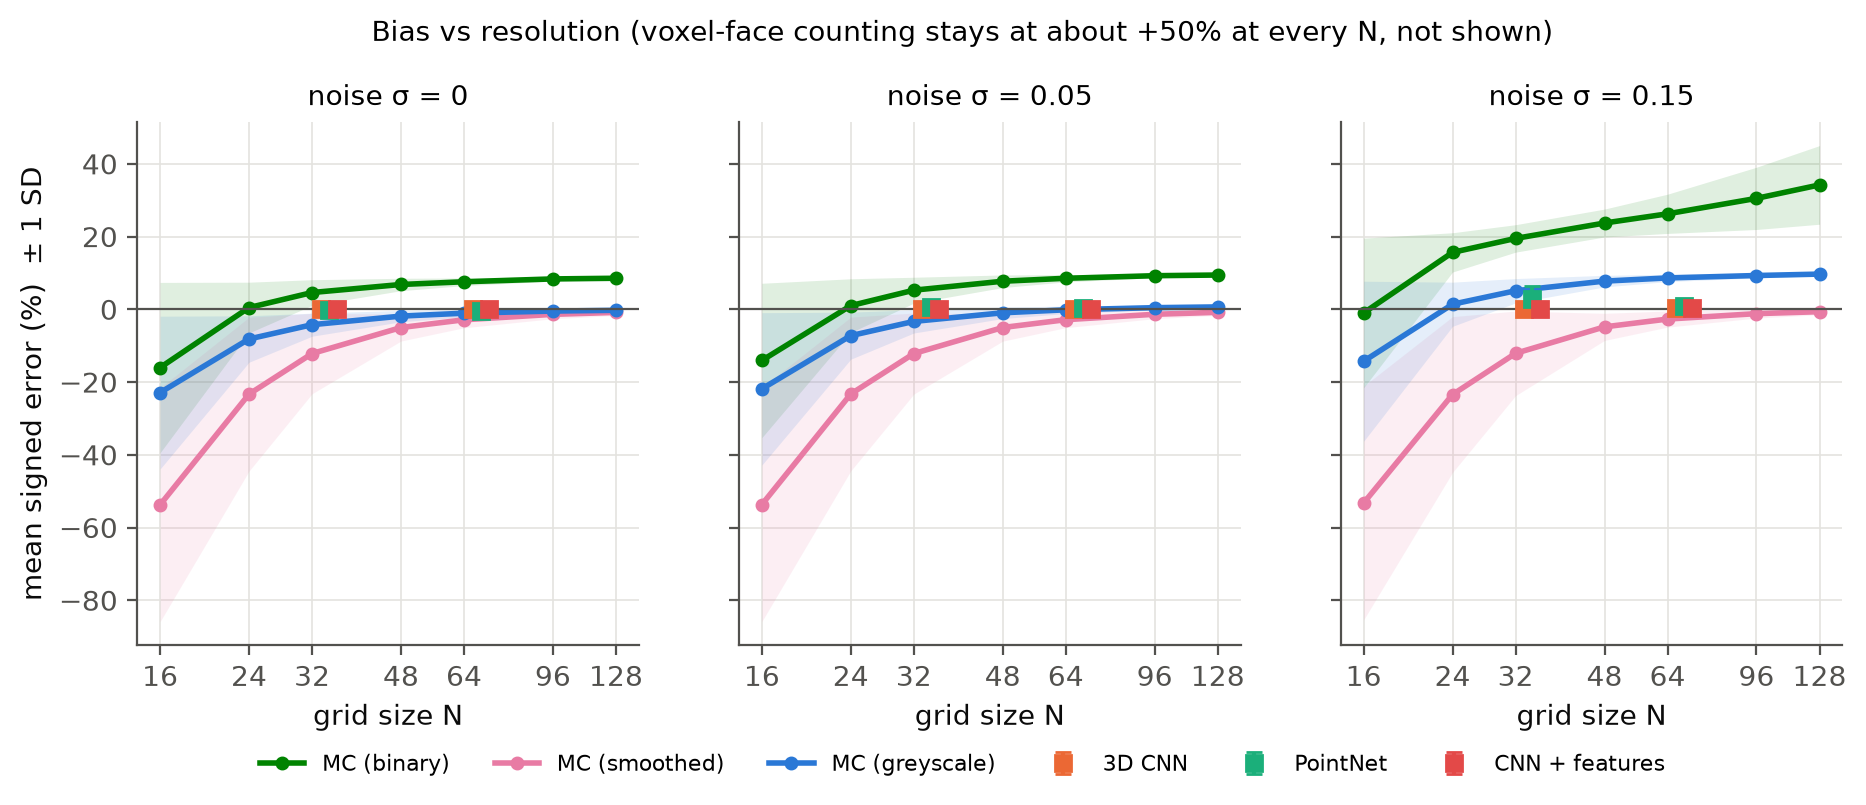
\includegraphics[width=\linewidth]{bias_vs_resolution.png}
  \caption{Mean signed error ($\pm$1 s.d.) of the marching-cubes estimators against grid size for 48
  test shapes. Learned models are shown at the two sizes they were trained on.}
  \label{fig:sweep}
\end{figure}

\subsection{Learned and calibrated corrections}
Every correction improves on raw greyscale marching cubes by a large factor. The lookup table already
reduces the test MAPE from 4.78\% to 2.97\% at $32^3$ and from 3.52\% to 0.79\% at $64^3$, so most of the
error at $64^3$ is a systematic, regime-dependent bias, while at $32^3$ it depends on the individual
object. The 3D CNN reaches 0.68\% and 0.26\%, a seven-fold and a thirteen-fold reduction, with a bias
within $\pm0.1\%$. The Random Forest performs almost identically at $32^3$ (0.72\%) and is the best
model at $64^3$ (0.18\%). Its most important inputs are the Euler number (0.29), the noise estimate (0.26), the smoothed-to-raw marching-cubes area ratio (0.22) and the face-count-to-marching-cubes area ratio (0.08).
The first two
measure exactly the two noise effects of Section~\ref{sec:theory}. PointNet is clearly weaker (1.98\%
and 1.04\%), because sampling points from a mesh that already contains the noise artefacts throws away
the intensity information the volume-based models use.

\subsection{Noise and object size}
The learned models are nearly insensitive to noise (Table~\ref{tab:noise}): at $64^3$ the CNN's MAPE
goes from 0.20\% on clean data to 0.40\% at $\sigma_n=0.15$, while greyscale marching cubes goes from
1.13\% to 8.56\%. Object size matters more than grid size. For objects less than 16 voxels across,
greyscale marching cubes has a MAPE of 6.43\%, the Random Forest 1.41\% and the CNN 1.24\%, the size
class where the CNN has its clearest advantage. Above 48 voxels the Random Forest reaches 0.08\%.

\begin{table}[t]
  \centering\footnotesize
  \caption{Test MAPE (\%) by resolution and noise level. Best per column in bold.}
  \label{tab:noise}
  \setlength{\tabcolsep}{3.5pt}
  \begin{tabular}{lrrrrrr}
    \toprule
    & \multicolumn{3}{c}{$32^3$} & \multicolumn{3}{c}{$64^3$} \\
    \cmidrule(lr){2-4}\cmidrule(lr){5-7}
    Method & $\sigma_n{=}0$ & $0.05$ & $0.15$ & $0$ & $0.05$ & $0.15$ \\
    \midrule
    Voxel faces & 44.10 & 45.64 & 80.38 & 48.31 & 49.91 & 98.40 \\
    MC (binary) & 5.24 & 5.85 & 20.05 & 7.64 & 8.49 & 27.34 \\
    MC (greyscale) & 4.73 & 3.84 & 5.77 & 1.13 & 0.86 & 8.56 \\
    MC (smoothed) & 13.87 & 13.82 & 13.65 & 3.11 & 3.09 & 2.93 \\
    \midrule
    MC + lookup & 3.06 & 3.05 & 2.80 & 0.84 & 0.83 & 0.71 \\
    Random Forest & 0.49 & 0.61 & 1.07 & \textbf{0.09} & \textbf{0.14} & \textbf{0.30} \\
    PointNet & 1.42 & 1.41 & 3.13 & 0.75 & 0.69 & 1.67 \\
    3D CNN & \textbf{0.46} & \textbf{0.55} & \textbf{1.02} & 0.20 & 0.19 & 0.40 \\
    \bottomrule
  \end{tabular}
\end{table}


\subsection{Unseen shape families and a failure case}
Both held-out families stay far below the classical errors (Fig.~\ref{fig:heldout}). On
superellipsoids, whose sharp edges do not occur in training, the CNN reaches 1.05\% and 0.45\% and the
Random Forest 0.73\% and 0.39\%, against 4.10\% and 3.38\% for greyscale marching cubes. Rough blobs are
the hardest case (CNN 1.96\%, Random Forest 1.71\% at $32^3$), with corrections biased low: the models
were trained on smooth shapes and cannot add back area hidden in sub-voxel roughness. At $64^3$ the
error falls to about 0.5\%.

The error distributions are heavy-tailed at $32^3$. The worst case is a test torus whose tube is 1.77
voxels thick: after blurring most of the tube stays below the iso-level, so greyscale marching cubes
recovers only 42 of its 142 voxel$^2$, and every model is off by 47\% to 66\%. A correction of the
marching-cubes area cannot recover a surface that is missing from the mesh.

\begin{figure}[t]
  \centering
  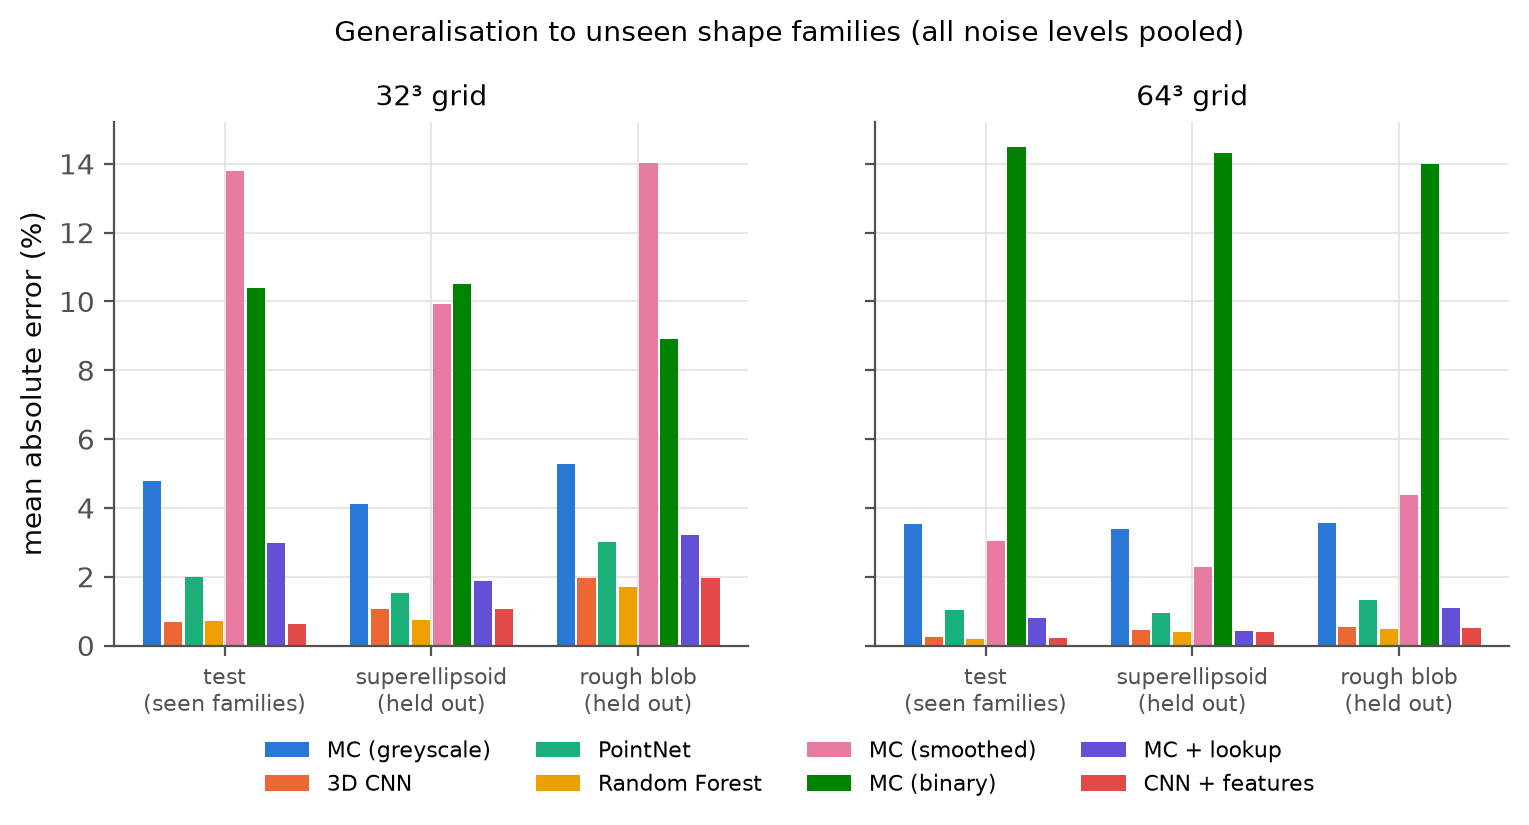
\includegraphics[width=\linewidth]{heldout_families.png}
  \caption{MAPE on the test split and on the two held-out families (all noise levels pooled).}
  \label{fig:heldout}
\end{figure}

\subsection{Which estimator to use}
Table~\ref{tab:regime} summarises when a learned correction is worth the effort. Its benefit is largest
where the classical methods are weakest: small objects, coarse grids and noisy data.

\begin{table}[t]
  \centering\small
  \caption{Recommended estimator by regime, based on the test results.}
  \label{tab:regime}
  \begin{tabular}{p{4.2cm}p{10cm}}
    \toprule
    Regime & Recommendation \\
    \midrule
    Any case & Do not use voxel-face counting or binary marching cubes for absolute area. \\
    Clean data, large objects & Greyscale marching cubes is within about 1\% at $64^3$. \\
    Noisy data ($\sigma_n=0.15$) & A learned correction (CNN or Random Forest) gives 0.3--1.1\%. \\
    Small objects ($<16$ voxels) & Use the 3D CNN (1.24\%, against 6.43\% for marching cubes). \\
    Thinner than about 2 voxels & No method tested here is reliable. \\
    \bottomrule
  \end{tabular}
\end{table}


\section{Conclusion}\label{sec:conclusion}
The errors of the classical surface-area methods are not random, and that is what makes them
correctable. Voxel-face counting is always about 50\% too high, binary marching cubes keeps an error that
does not shrink with resolution, and greyscale marching cubes is pulled down on curved surfaces, by an
amount a simple blurring argument predicts, and pushed up by noise.

A correction learned from synthetic shapes with known area removes most of this error. On test shapes
it cuts the error of greyscale marching cubes from 4.78\% to 0.68\% at $32^3$ and from 3.52\% to 0.18\% at
$64^3$, barely changes with noise, and stays below 2\% on shape families never seen in training. A
Random Forest on ten simple measurements does as well as a 3D CNN with 3.6 million parameters; the CNN
is worth its extra cost mainly for small objects on coarse grids. Structures thinner than about two
voxels and roughness smaller than one voxel remain out of reach, because the information is no longer
in the image. Natural next steps are a more realistic CT simulation, volumes with many touching
structures, and a test on a real scan of an object with a known surface area.


\section{Limitations}\label{sec:limitations}
\begin{itemize}\setlength\itemsep{1pt}
  \item \textbf{Simplified physics.} Noise is white and added in the image domain; real CT noise is
        correlated and signal dependent, and real volumes have beam-hardening, ring and streak artefacts.
  \item \textbf{One isolated object per volume.} Porous media and lattices with many touching
        structures are untested.
  \item \textbf{Fixed acquisition.} Two grid sizes, three noise levels and a fixed blur; behaviour
        outside this range is untested.
  \item \textbf{Sub-voxel roughness.} On rough surfaces the correction is a learned prior, not a
        measurement.
  \item \textbf{Limited shapes, no tuning.} Training shapes are star-shaped or of genus one; there was
        no hyperparameter tuning, each model was trained once, and the $64^3$ CNN only for 15 epochs.
  \item \textbf{No real scan.} No measurement on a real CT scan with a known surface area is included.
\end{itemize}


\section*{Code and Data Availability}
Code, trained weights and result tables are in the project repository; the dataset is fixed by its
generation script and seed (51) and is shared alongside the code.

\appendices
\section{Curvature bias of greyscale marching cubes}\label{app:curvature}
For a plane and a symmetric blur the
$0.5$ iso-surface of the blurred image coincides with the true surface. For a curved surface it does
not. If the effective blur is Gaussian with variance $\sigma_\text{eff}^2$, the level sets of the
blurred indicator move towards the centre of curvature by
\begin{equation}
  \delta \approx \sigma_\text{eff}^2\,H, \qquad H = \tfrac12(\kappa_1+\kappa_2),
  \label{eq:shift}
\end{equation}
where $H$ is the mean curvature. The intuition is that blurring a curved object spreads its intensity
outwards over a larger volume, so the half-intensity surface ends up slightly inside the true one, and
more so where the surface bends sharply. (Formally this follows from the heat equation, since Gaussian
blurring is diffusion for a time $\sigma_\text{eff}^2/2$.) For a sphere of radius $R$ this gives a relative area error of
$-2\delta/R = -2\sigma_\text{eff}^2/R^2$. In our forward model the voxel box ($\sigma^2 = 1/12$) and the
Gaussian PSF ($\sigma = 0.6$) combine to $\sigma_\text{eff}^2 \approx 0.443$ voxel$^2$; adding a
smoothing filter with $\sigma_s = 1$ raises it to $1.443$. Table~\ref{tab:curvature} compares this
prediction with the measured errors on clean spheres. The agreement is close at low resolution, where
the curvature term dominates; at $64^3$ the remaining discrepancy is of the same size as the
interpolation error of marching cubes itself.

\begin{table}[h]
  \centering\footnotesize\setlength{\tabcolsep}{3pt}
  \caption{Greyscale marching-cubes error on clean spheres: measured vs the curvature prediction
  $-2\sigma_\text{eff}^2/R^2$ from Eq.~\eqref{eq:shift}. $R$ in voxels.}
  \label{tab:curvature}
  \begin{tabular}{rrrrrr}
    \toprule
    & & \multicolumn{2}{c}{MC on greyscale} & \multicolumn{2}{c}{MC after smoothing ($\sigma_s=1$)}\\
    \cmidrule(lr){3-4}\cmidrule(lr){5-6}
    Grid & $R$ & predicted & measured & predicted & measured \\
    \midrule
    $16^3$ & 5.4  & $-3.04\%$ & $-3.65\%$ & $-9.90\%$ & $-10.99\%$ \\
    $32^3$ & 12.6 & $-0.56\%$ & $-0.62\%$ & $-1.82\%$ & $-2.00\%$ \\
    $64^3$ & 27.0 & $-0.12\%$ & $-0.05\%$ & $-0.40\%$ & $-0.43\%$ \\
    $128^3$ & 55.8 & $-0.03\%$ & $+0.07\%$ & $-0.09\%$ & $-0.10\%$ \\
    \bottomrule
  \end{tabular}
\end{table}

\section{Reference surface areas}\label{app:reference}
Spheres, cylinders and tori have closed-form areas. For an ellipsoid with semi-axes $a\ge b\ge c$,
\begin{equation}
\begin{aligned}
  A &= 2\pi c^2 + \frac{2\pi ab}{\sin\varphi}\left[E(\varphi,m)\sin^2\varphi + F(\varphi,m)\cos^2\varphi\right],\\
  \cos\varphi &= \frac ca,\qquad m = \frac{a^2(b^2-c^2)}{b^2(a^2-c^2)},
\end{aligned}
\end{equation}
with $F$ and $E$ the incomplete elliptic integrals of the first and second kind. The remaining
families (random blobs and superellipsoids) are star-shaped, i.e.\ their surface is
$\{r(\mathbf u)\,\mathbf u : |\mathbf u|=1\}$ for a radial function $r$. We triangulate them by mapping
the vertices of a subdivided icosahedron to radius $r(\mathbf u)$. For a smooth surface the area of such
an inscribed mesh converges as $A_\ell = A + c\,h_\ell^2 + o(h_\ell^2)$ in the edge length $h_\ell$, and
each subdivision halves $h_\ell$, so Richardson extrapolation of two levels,
\begin{equation}
  A_\text{ref} = \tfrac13\left(4A_{\ell+1} - A_\ell\right),
\end{equation}
cancels the leading error term. We use levels 6 and 7 (81,920 and 327,680 triangles) and keep
$|A_\text{ref}-A_7|$ as an error estimate for each shape.


\bibliographystyle{IEEEtranN}
\bibliography{refs}

\end{document}
